\subsection{Opis hipotezy}\label{opis-hipotezy}

\textbf{Numer:} 10\\\textbf{Nazwa:} Wypadki a rodzaj
drogi\\\textbf{Treść:} Na autostradach będzie mało wypadków, ponieważ są
one bezpiecznymi drogami - obowiązuje na nich nieskomplikowany sposób
poruszania się, nie ma skrzyżowań, oraz mieszkańcy USA i WB są
przyzwyczajeni do częstego korzystania z nich. Ponadto nie poruszają
się~po nich piesi. Natomiast więcej wypadków może pojawić się na drogach
o randze porównywalnej z polskimi krajowymi oraz wojewódzkimi
(Principal, Major), ponieważ~z jednej strony mogą mieć skomplikowana
infrastrukturę co może wymagać~więcej umiejętności od kierowców, a z
drugiej pozwalają osiągnąć znaczne prędkości. Możliwe jest też
zaobserwowanie znacznej ilości wypadków śmiertelnych na drogach
drugorzędnych (Minor), ponieważ często na terenach wiejskich ludzie
dopuszczają się bardziej brawurowej jazdy i kierowania po spożyciu, gdyż
rzadziej można tam spotkać funkcjonariuszy drogówki.

\subsection{Wyniki związane z
hipotezą}\label{wyniki-zwiazane-z-hipoteza}

\textbf{Rodzaj drogi}

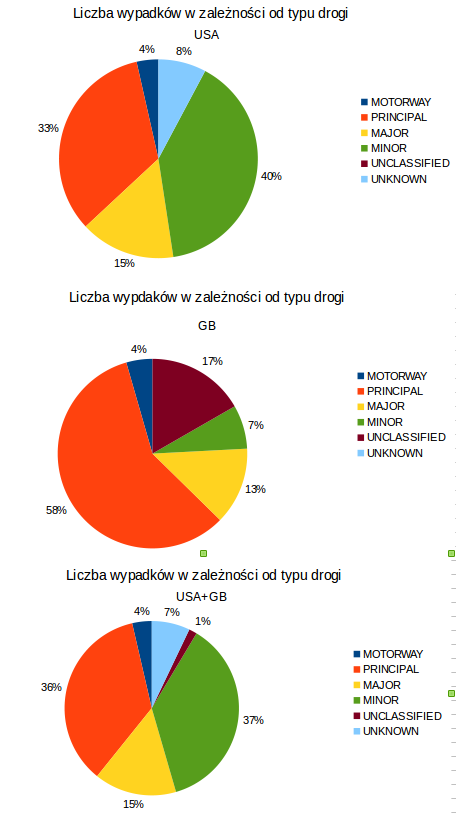
\includegraphics[width=0.8\textwidth]{images/statistics/road_type.png}

Hipoteza potwierdziła się, na autostradach obserwuje się niewiele
wypadków śmiertelnych w porównaniu do innych typów drogi. Tutaj
instnieje spore podobieństwo pomiędzy USA a WB. Natomiast w przypadku
innych rodzajów dróg pojawiają się duże rozbieżności, choć wyniki te
potwierdzają prawdziwość hipotezy. W WB wypadki śmiertelne częściej
spotykane są na drogach krajowych, podczas gdy w USA spora część tego
udziału przypada drogom drugorzędnym. Może to wynikać z udziału
poszczególnych typów dróg w infrastrukturze danego kraju, lub
rozbieżności w ich klasyfikacjach.
